\documentclass[a4paper]{article}
\usepackage[utf8]{inputenc}
\usepackage[spanish, es-tabla, es-noshorthands]{babel}
\usepackage[table,xcdraw]{xcolor}
\usepackage[a4paper, footnotesep = 1cm, width=20cm, top=2.5cm, height=25cm, textwidth=18cm, textheight=25cm]{geometry}
%\geometry{showframe}

\usepackage{tikz}
\usepackage{amsmath}
\usepackage{amsfonts}
\usepackage{amssymb}
\usepackage{float}
\usepackage{graphicx}
\usepackage{caption}
\usepackage{subcaption}
\usepackage{multicol}
\usepackage{multirow}
\setlength{\doublerulesep}{\arrayrulewidth}
\usepackage{booktabs}

\usepackage{hyperref}
\hypersetup{
    colorlinks=true,
    linkcolor=blue,
    filecolor=magenta,      
    urlcolor=blue,
    citecolor=blue,    
}

\newcommand{\quotes}[1]{``#1''}
\usepackage{array}
\newcolumntype{C}[1]{>{\centering\let\newline\\\arraybackslash\hspace{0pt}}m{#1}}
\usepackage[american]{circuitikz}
\usetikzlibrary{calc}
\usepackage{fancyhdr}
\usepackage{units} 

\graphicspath{{../Ejercicio-1/}{../Ejercicio-2/}{../Ejercicio-3/}{../Ejercicio-4/}}

\pagestyle{fancy}
\fancyhf{}
\lhead{22.01 Teoría de Circuitos}
\rhead{Mechoulam, Lambertucci, Rodriguez Turco, Londero, Galdeman}
\rfoot{\centering \thepage}

\begin{document}

\subsection{Celda universal}
Las celdas universales es un conjunto de filtros RC activos de segundo orden, compuestos por amplificadores operacionales configurados de forma sumadora, restadora, integradora, amplificadora o atenuadora, puestos en cascada. Estas son también conocidas como celdas de variables de estado, debido al uso de dicho método para la resolución de las ecuaciones diferenciales. Este tipo de celdas se caracteriza por poseer bajas sensibilidades con respecto a sus componentes, alta flexibilidad y buen rendimiento. Existen distintos tipos de configuraciones, donde cada una de estas posee sus respectivas ventajas y desventajas. A continuación, se procede a analizar cada una de ellas\footnote{L. Huelsman, Active and passive analog filter design, 2nd ed. New York: McGraw-Hill, 1993.}
%\footnote{R. Raut and M. N. S. Swamy, Modern Analog Filter Analysis and Design, 1st. ed. New York: McGraw-Hill, 1993.}.

\subsubsection{Kerwin-Huelsman-Newcomb (KHN)}
La celda Kerwin-Huelsman-Newcomb, nombre otorgado a partir de sus creadores\footnote{W. J. Kerwin, L. P. Huelsman and R. W. Newcomn, ``State-Variable Synthesis for Insensitive Integrated Circuit Transfer Functions  IEEE Journals \& Magazine'', Ieeexplore.ieee.org, 2019. [Online]. Available: \url{https://ieeexplore.ieee.org/document/1049798}. [Accessed: 20- Oct- 2019].}, puede ser comprendida con mayor facilidad a partir de un ejemplo. Se considera una transferencia de un filtro pasabanda:
\begin{equation}
	\frac{V_o(s)}{V_i(s)} = \frac{Ks}{s^2 + a_1 s + a_0}
\end{equation}

Se divide, tanto el numerador como el denominador de la expresión de la izquierda, por $s^2$
\begin{equation}
	\frac{V_o(s)}{V_i(s)} = \frac{\frac{K}{s}}{1 + \frac{a_1}{s} + \frac{a_0}{s^2}}
	\label{equ:1}
\end{equation}

Siendo
\begin{equation}
	V_a(s) = frac{V_i(s)}{1 + \frac{a_1}{s} + \frac{a_0}{s^2}}
	\label{equ:2}
\end{equation}

Y reescribinedo (\ref{equ:1}), se obtiene
\begin{equation}
	V_o(s) = \frac{K}{s} \cdot V_a(s)
	\label{equ:3}
\end{equation}

Si se utiliza la transformada de Laplace inversa tanto en (\ref{equ:2}) como en (\ref{equ:3}), se observa que se posee
\begin{equation}
\begin{split}
	v_a(t) =\ v_i(t) - a_1 & \int v_a(t)dt - a_0 \int \left( \int v_a(t)dt \right) dt \\
	v_o(t) =& \ K\int \left( \int v_a(t)dt \right) dt
\end{split}
\end{equation}

Del sistema anterior, $v_a(t) = \ddot{x}(t) $, $\int v_a(t)dt = \dot{x}(t)$ y $\int \left( \int v_a(t)dt = x(t) \right) dt$ son las llamadas variables de estado. Es más fácil de interpretar estas observando la Figura (\ref{fig:block}).

\begin{figure}[H]
\centering
	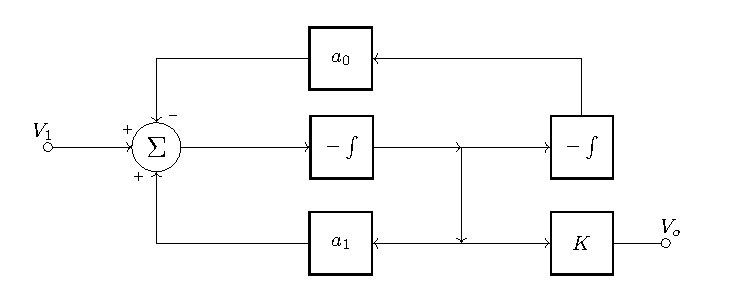
\includegraphics[width=0.6\textwidth]{ImagenesEjercicio4/Diagrama-De-Bloques.pdf}
	\caption{Diagrama de bloques de la celda KHN.}
	\label{fig:block}
\end{figure}

Es así que, para cada integrador se obtiene $V_{o3} = \frac{-V_{o2}}{sR_2C_2}$ y
$V_{o2} = \frac{-V_{o1}}{sR_1C_1}$, mientras que para el sumador
\begin{equation*}
	V_{o1} = -\frac{R_6}{R_5} V_{o3} + \frac{R_4}{R_3 + R_4} \frac{R_5 + R_6}{R_5} V_1 + \frac{R_3}{R_3 + R_4} \frac{R_5 + R_6}{R_5} V_{o2}
\end{equation*}

Finalmente, con las definiciones previas se puede elaborar el circuito presentado a continuación:
\begin{figure}[H]
\centering
	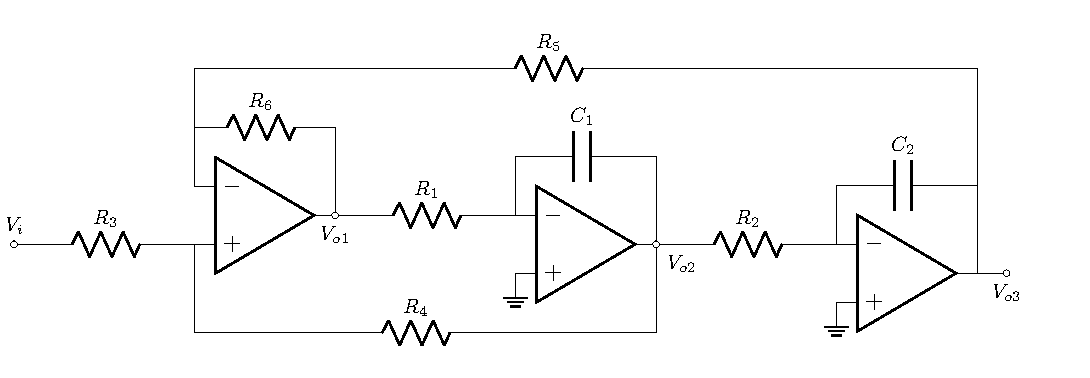
\includegraphics[width=0.9\textwidth]{ImagenesEjercicio4/KHN.pdf}
	\caption{Celda KHN.}
	\label{fig:KHN}
\end{figure}

\subsubsection{Tow-Thomas}

\subsubsection{Ackerberg-Mossberg}

\subsubsection{Fleischer-Tow}

\end{document}
